\documentclass[11pt]{report}
\usepackage{standalone}
\graphicspath{ {images/} }
\setcounter{tocdepth}{5}
\setcounter{secnumdepth}{5}
\usepackage{natbib}
\bibliographystyle{agsm}
\usepackage{etoolbox}
\setlength{\parindent}{0em}
\setlength{\parskip}{0.25em}
\usepackage[raggedright]{titlesec}
\usepackage{hyperref}
\usepackage{capt-of}
\patchcmd{\bibliography}{\section*}{\section}{}{}
\titlespacing*{\chapter}{0pt}{-40pt}{10pt}
\titleformat{\chapter}[block]{\normalfont\huge\bfseries}{\thechapter}{15pt}{}
\usepackage{rotating}
\usepackage[titletoc]{appendix}
\usepackage{pgfgantt}
\usepackage{graphicx, rotating, caption, lscape, threeparttable}% \usepackage{amsmath}
\usepackage{array}
\usepackage{pdflscape}
\usepackage{geometry}
\usepackage{listings}
\usepackage[T1]{fontenc}
\usepackage{amssymb}
\usepackage{textcomp}






\begin{document}
\chapter{Design}

\section{Design Methodology}

The design and implementation of the System were approached using a top-down design methodology. The top-down design was chosen due to the benefits it encourages in the development of the product such as; 

\begin{itemize}
\item Modularization - The System structure is well defined and concerns are separated allowing for ease of testing and code reuse for increased extensibility.  

\item Readability - The System can be easily understood resulting in a reduced surface area for unexpected behaviour within the System as bugs which disrupt the readability of the system can be readily identified.
\end{itemize}
The overall problem of visualizing sentiment analysis was then broken down into smaller components each of which were broken down further until the components discovered could not be broken down anymore. Figure \ref{fig:top-down} shows the process of how this was executed in-depth.

\section{System Architecture}
The high-level system structure identified using top-down design finalized the following set of components; scraper, preprocessing framework, classifier framework and a visualizer. Having multiple subsystems allowed for a separation of concerns and aided in the development of the System pipeline.  The System component responsibilities are as follows:

\begin{itemize}
\item Scraper: Responsible for Tweet Collection and creation of composite day objects that represent the tweet count for a given day.
\item Preprocessing Framework: Responsible for the tokenization of tweets.
\item Classifier Framework: Responsible for configuring classifiers and classifying tweets against configured Classifiers. The Classifier framework also creates composite day objects that represent the classification count for a given day.
\item Visualizer: Responsible for the API calls the visual website component will utilize.
\end{itemize}
The components and their interactions can be visualized using Figure  \ref{fig:component}.
\\

\begin{landscape} 
  \hspace*{0cm}
  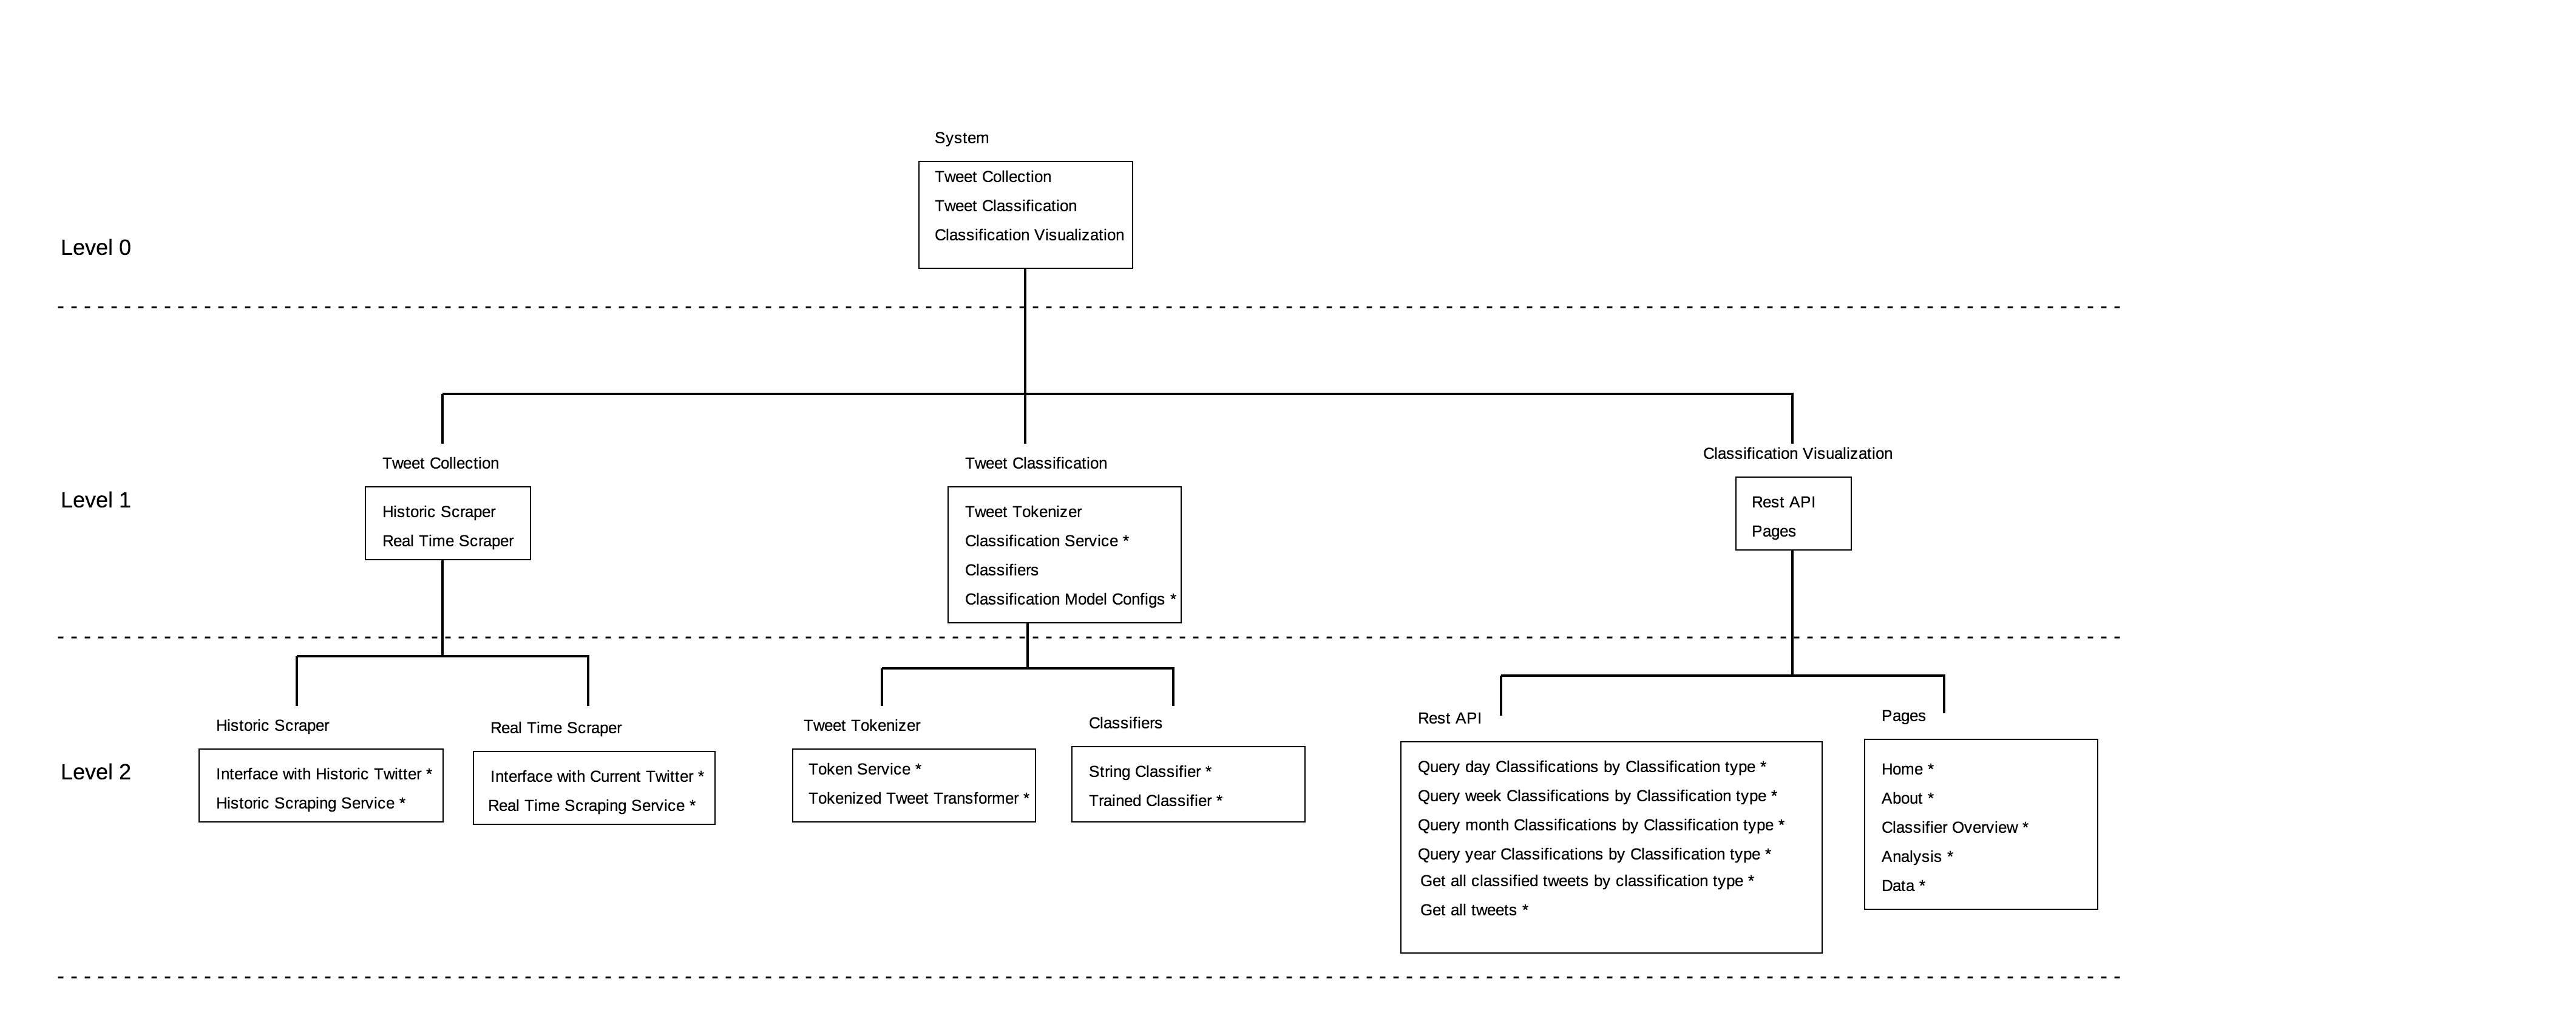
\includegraphics[width=22.5cm,height=12cm]{images/top-down-final.png}
  \captionof{figure}{Top Down Design Approach.}
  \label{fig:top-down}        
\end{landscape}


\begin{landscape}
\begin{center}
  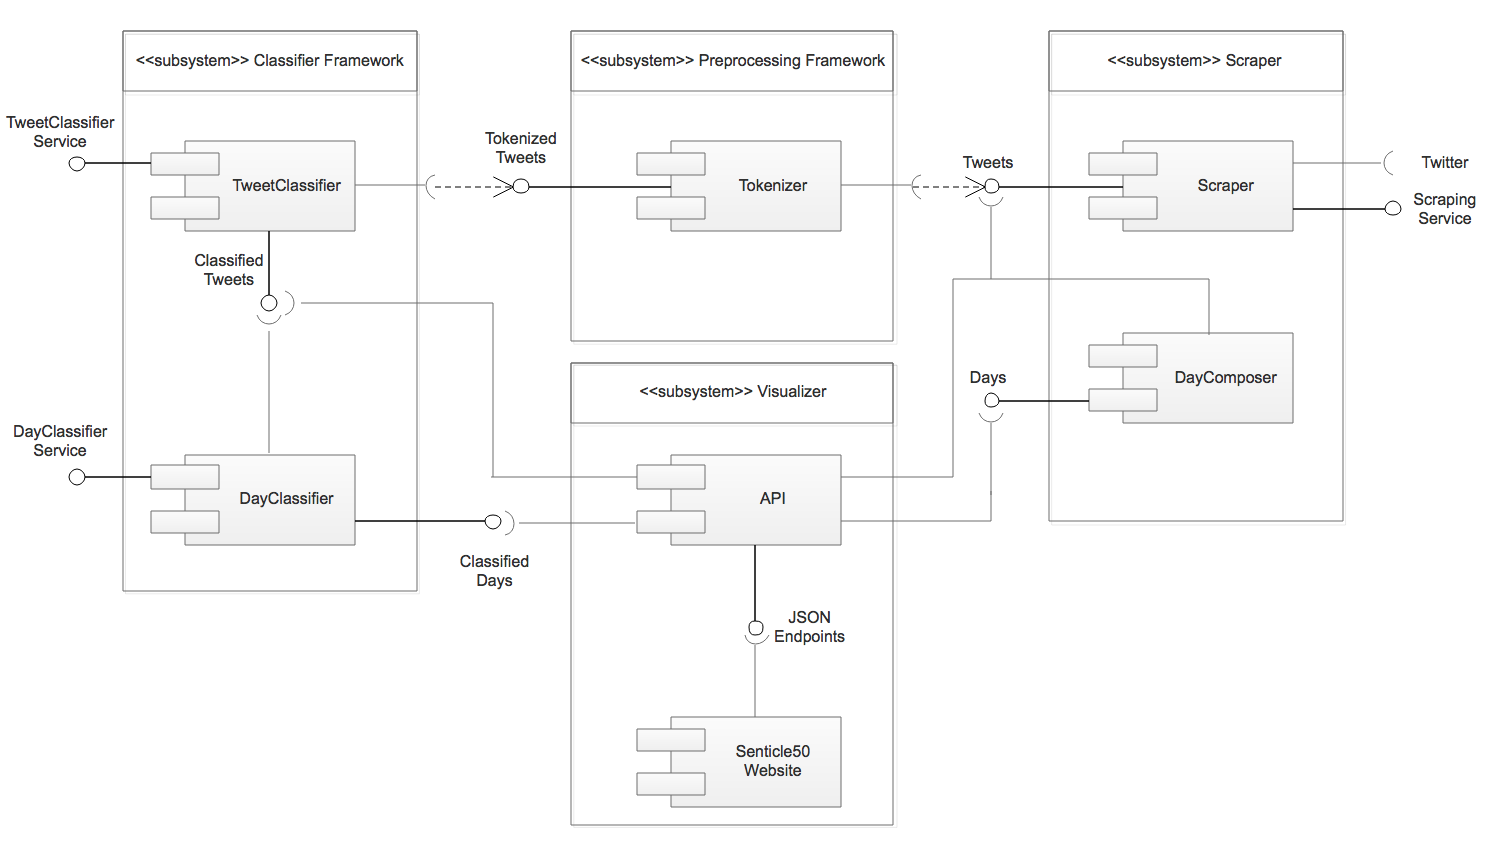
\includegraphics[width=\linewidth]{images/component-diagram.png}
  \captionof{figure}{Component diagram.}
  \label{fig:component}
\end{center}
\end{landscape}

\section{Classifier Architecture}
The System is architected in such a way to split the model from the classifier itself as well as an interface structure which enforces each classifier implements the base required classifier methods. Having this structure allows for a number of beneficial qualities as listed below.

\begin{center}
  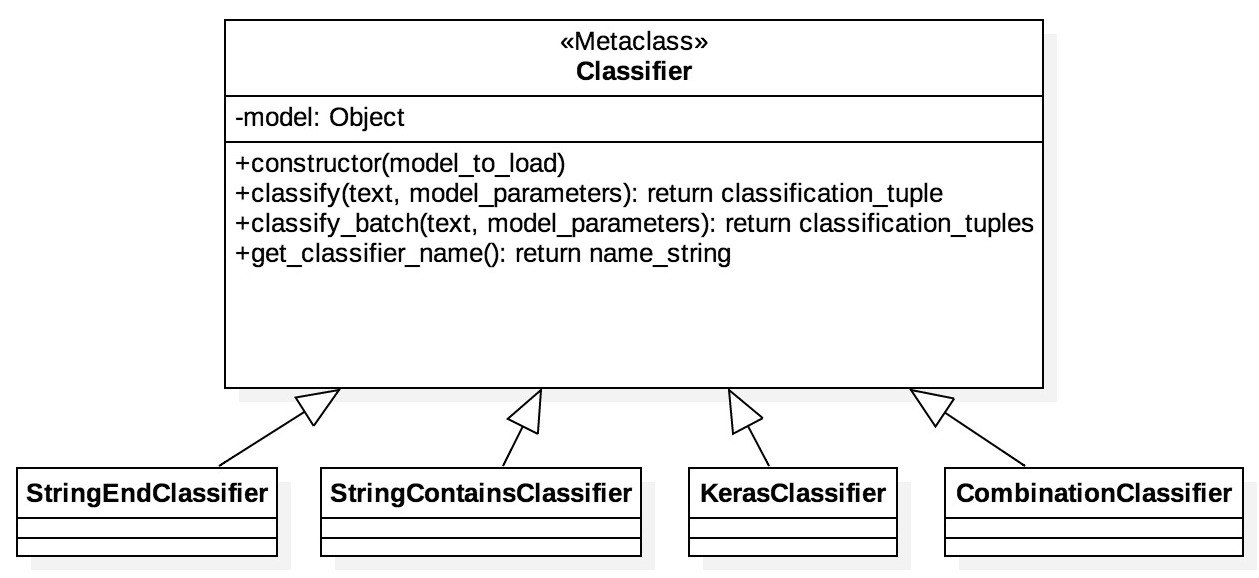
\includegraphics[width=12cm]{images/classifier-inheritance.jpg}
  \captionof{figure}{Classifier Interface Structure.}
  \label{fig:classifier-interface}
\end{center}

\subsection*{Generic Classifiers}
Classifiers are unique to the model type they can serve, the classifier classes are placeholder classes for the model i.e. a model is an attribute of a classifier and thus one classifier class can serve multiple models of the same base model type.

\subsection*{Pluggable Classifiers}
The System structure of multiple classifiers implementing methods from the base classifier object ensures that new class implementations of a classifier can be implemented and plugged into the classification framework at ease.

For a new classifier to be plugged into the framework it must include:
\begin{itemize}
\item a constructor taking the model attribute to classify against.
\item a classify method to classify one tweet.
\item a batch classify method for classifying batches of tweets.
\item a get method to return the classifier name for storage in the classifier registry.
\end{itemize}

\section{Database Schema}
The System as identified in the analysis and specification required a database to permanently store the sentiment analysis that it has computed. The architectural process undertaken to design the database was to first use the analysis of related systems to list data that is expected in this system. After all the data was listed, entities were extracted such as ``Tweet''. Each entity had it's corresponding attributes extracted. 

\subsubsection*{Modelling the Data}
The database now had a preliminary design where each of the entities was representative of the database tables. The entities were first modelled first using a conceptual data model to solidify the relations between each of the tables and the attributes which belonged to each relation. The conceptual model was then converted to a physical model to gain an understanding of the attribute key relations and the types required to model each attribute within a physical database.

\subsubsection*{Normalization}
The list of tables that were modelled using the physical and conceptual models was normalized to Boyce-Codd Normal Form \citep*{CoddRecentInvestigationsRelational1974} to prevent data redundancy and undesired database behaviour i.e. insertion, deletion or update anomalies.
\\

The normalization of the schema required that for each table R within the designed database, BCNF(R) holds true such that for every functional dependency of R i.e. X\textrightarrow Y (where attribute Y depends on the value of X) either of the following conditions must be true;

\begin{itemize}
\item X\textrightarrow Y is a trivial functional dependency ($Y  \subseteq X$) 
\item X is a superkey (set of attributes within a table whose values can be used to identify a unique record) of table R
\end{itemize}

The result of applying BCNF to the preliminary database design was the creation of more tables e.g. the table ``Label'' was extracted out of ``Classified\textunderscore Tweet'' into its own table due to its functional dependency on `\texttt{Classification\textunderscore Type} and not \texttt{Classified\textunderscore Tweet.Id}. The resulting changes to the database were amended within the database models and thus the final conceptual and physical database structure can be viewed by Figure \ref{fig:conceptual-erd} and Figure \ref{fig:physical-erd}.




\newgeometry{a4paper,left=1in,right=1in,top=1in,bottom=1in,nohead}
\begin{landscape} 
\begin{center}
  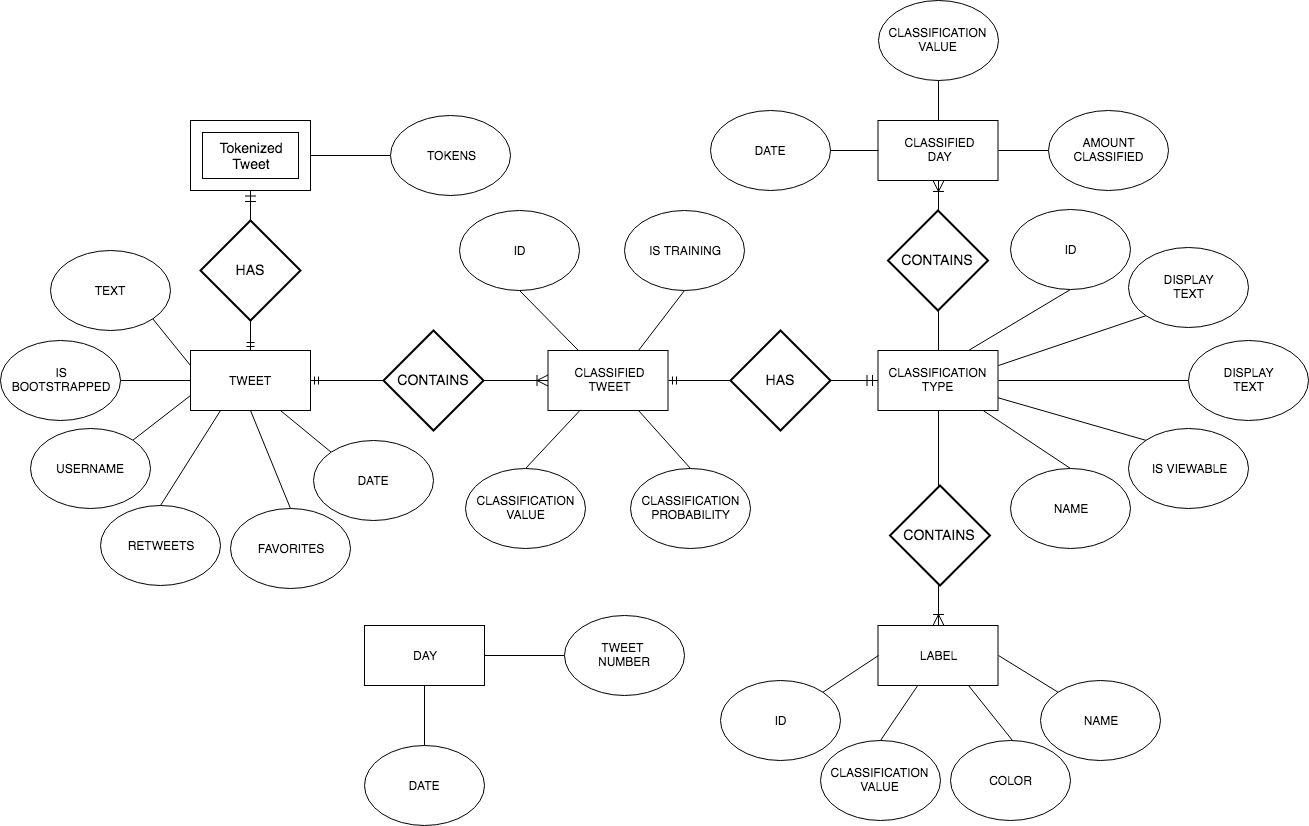
\includegraphics[width=22cm]{images/conceptual-erd.jpg}
  \captionof{figure}{Conceptual Entity-Relationship Diagram.}
  \label{fig:conceptual-erd}
\end{center}
\end{landscape}

\begin{landscape} 
\begin{center}
  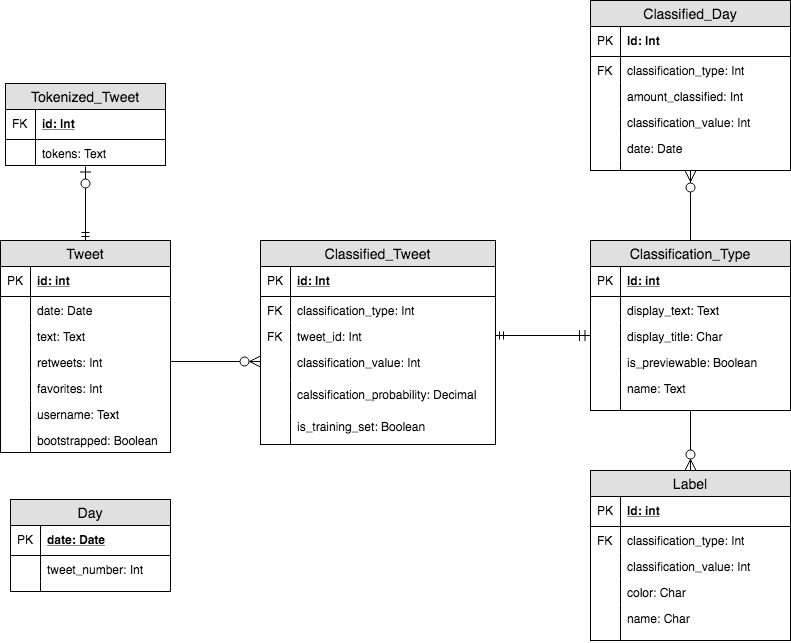
\includegraphics[width=\textwidth]{images/physical-erd.jpg}
  \captionof{figure}{Physical Entity-Relationship Diagram.}
  \label{fig:physical-erd}
\end{center}
\end{landscape}
\restoregeometry % Restore the global document page margins

\clearpage

\section{Design Patterns}

\subsection*{Registry Pattern}
As mentioned each classifier is a separate class and therefore to enable a generic service to decide which Classifier to use when given a configuration file the rationale was taken to design a  \textbf{Classifier Registry} that on-load of the System registers all of the classifiers classes which are available in the System. The registry can then be used to retrieve the class file of a requested Classifier in the system.

\subsection*{Handler Service Transformer Pattern}
For each of the background operations, the system handles the operation request through a handler which calls a service that utilizes a transformer to convert computed attributes into an object form readable by the System.

Each layer in an operation therefore has set responsibilities and can be summarized as follows:

\begin{itemize}
\item Handler: Calls services required with their respective parameters
\item Service:  Encapsulates the business logic and the utilization of a transformer class to convert it's computed attributes
\item Transformer: Converts parameters into a System object.
\end{itemize}

\section{Models}
\subsection{Naive Brexit Stance Model}
The Naive Brexit Stance Model was designed to determine a tweet as having ``Leave'' or ``Remain'' sympathies towards the topic of ``Britain Leaving the European Union''. The model was trained using tweets ending in leave or remain hashtags based off of previous work in the Sheffield System  \citep{maynard_framework_2017}. See Table \ref{table:naive-labels} for the specific class labels from which the classifier learnt natural language patterns unique to the mutually exclusive leave and remain sides of the discussion.
\\

\textit{N.B. It's naivety lies in the absence of using sentiment when classifying a tweets stance
(see Brexit stance for how sentiment can be used to further improve stance detection)}

\clearpage

\begin{center}
\begin{tabular}{ |p{1.5cm}||p{5cm}| }
\hline
 Class & Label\\
 \hline
 Leave &  \#VoteLeave \#LeaveEU\\
 \hline
 Remain &  \#StrongerIn, \#VoteRemain\\
 \hline
\end{tabular}
\captionof{table}{Naive Brexit Model Labelling}
\label{table:naive-labels}
\end{center}

\subsection{Sentiment Model}
The Sentiment Polarity Model was designed to determine a tweet as being ``Positive'' or
``Negative'' sentiment using the textual content of the tweet. The distant labelling technique
chosen for use within this model was the use of distant plain-text emoticon labels i.e. tweets
that contain positive emoticons and no negative emoticons and vice versa (see Table  \ref{table:sentiment-labels} for the specific class labels). Using this distant labelling technique within the training it learnt natural language patterns unique to positive
and negative tweets that aided in classifications.

\begin{center}
\begin{tabular}{ |p{1.5cm}||p{5cm}| }
\hline
 Class & Label\\
 \hline
 Positive & ":)", ":-)", ": )", ":D", "=)"\\
 \hline
 Negative &  ":(", ":-(", ": ("\\
 \hline
\end{tabular}
\captionof{table}{Sentiment Model Labelling}
\label{table:sentiment-labels}
\end{center}

\subsection{Brexit Stance Model}
The Brexit Stance model uses a tweets classifications from the Naive Brexit Stance and
Sentiment models to identify it as having Leave or Remain sympathies.
\\

The model maps the positive sentiment tweets to the Brexit stance it was identified as
(using the Naive Brexit Stance model) and the negative sentiment tweets to the opposite
stance from which it was originally identified as (using the Naive Brexit Stance model).
\\

This classifier therefore acts on the assumption that a tweet that is classified as having
contents regarding one side of the Brexit Debate does not support that side if the sentiment
of the tweet is negative and thus classifies negative tweets to the opposite side from which
it was originally identified.

\clearpage

\section{System Pipeline}
The main high-level operation of visualizing the sentiment analysis of tweets within real time requires that collected tweets pass through the components provided by the System in a chronological order and thus as part of design a System pipeline was conceived. The pipeline is traversed by each tweet collected and can be visualized using Figure \ref{fig:syspipe}.

\begin{center}
  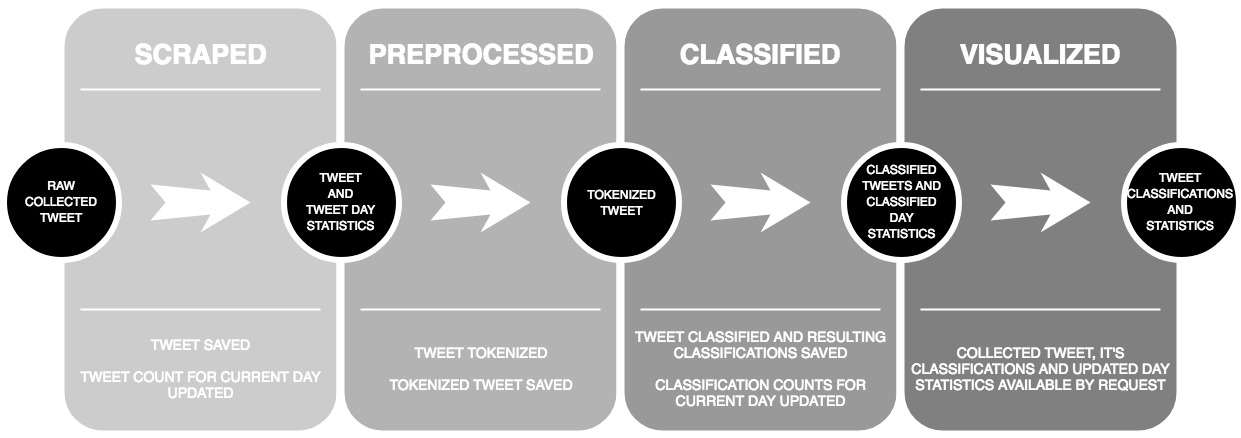
\includegraphics[width=\textwidth]{images/syspipe.jpg}
  \captionof{figure}{System Pipeline.}
  \label{fig:syspipe}
\end{center}

\section{Constraint Resolution}

The project as previously identified in the Specification has a number of limiting/constraint factors that were considered in the design of the system. 

\subsection*{Execution Time} 

\subsubsection*{Concurrent Tasks}
The System within its high-level operations will repeatedly perform the same task on each input i.e. for tokenization each tweet will undergo the same series of tokenization steps. This repetition is an ideal candidate for concurrent activity which fuelled the design behind utilising a thread pool executor to perform tasks in the system which can occur concurrently. The System therefore allows for the specification of worker threads within the system operations that use a thread pool to result in a linear decrease of execution time as thread numbers increase.

\subsubsection*{Asynchronous Tasks}
The System contains actions that are time-consuming to execute and the result of such actions is not needed by the caller of the actions themselves i.e. the saving of items to the database. Having to wait for these operations to occur despite not needing the result can slow down the overall execution of the system. The System combats these tasks by executing them asynchronously in the background allowing for the system to carry on processing and not wait for execution of such tasks.

\subsubsection*{Live Processing}
The System's visual component requires access to tweet count and classification statistics which will be requested via HTTP GET requests. The execution time of calculating statistics such as a sum or maxima grows exponentially with the volume of data on which the statistic is being calculated and as a consequence is unsustainable for serving HTTP requests in a timely manner (on an ever-growing dataset). Therefore the system design incorporates composite objects for statistics which describe the statistics of tweet count and classification count for each classifier on a day granularity. The number of records involved in a statistic calculation is therefore reduced to the number of days in the given time period opposed to the number of tweets. By utilizing composite objects the system execution time for live processing is significantly reduced when serving HTTP requests.

\subsection*{External Storage Size} 
The System will potentially accept up to thousands of tweets per day, it is therefore important that the storage and processing of this data do not occupy too much space. To approach this, the system's relational database schema was designed to be in normalized form and therefore minimize data redundancy by having data records only stored once and related via relations i.e. a tweet is only stored once with a primary key to which related tables use as a foreign key reference. The system also conserves memory by ensuring that only data required by the system is stored i.e. a tweet is stored as a reduced model of the raw input of a tweet (containing only the core details required for the system to operate).

\enlargethispage{\baselineskip}
\enlargethispage{\baselineskip}
\subsection*{Tradeoff Resolution} 

Execution Time vs RAM: The System must strive to be as efficient in time as possible but must beware of the tradeoff with RAM such that operations must be timely but not deplete the system of too much memory resource. To combat this, system features which operate on large amounts of data have been designed to be processed in batches. The Batch processing allows for the system to scale its batch size based on the specifications of the host system it is operating on and thus provides a compromise between Execution Time and RAM that maximizes the efficiency of the system.

\end{document}